\chapter{Результаты анализа коллективной анизотропии}

\section{Результаты анализа экспериментальных данных HADES}

\subsection{Направленный поток $v_1$ протонов как функции быстроты и поперечного импульса в столкновениях Au + Au и Ag + Ag}

На рис.~\ref{fig:hades_prl} приведен направленный поток $v_1$ протонов рожденных в столкновениях ядер золота при кинетической энергии пучка $E_{kin}=1.23A$~ГэВ как функция быстроты и поперечного импульса.
Результатом данной работы является систематическая ошибка в связи с непотоковым корреляциями, которая позволила коллаборации опубликовать данные.
%
\begin{figure}[ht]
\begin{center}
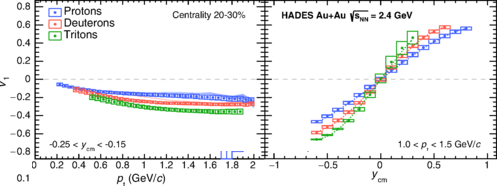
\includegraphics[width=0.75\linewidth]{images/HADES_prl.png}
\caption{Направленный поток ($v_1$) протонов, дейтронов и тритонов  рожденных в столкновении Au+Au при энергии $E_{kin}=$1.23$A$~ГэВ как функция быстроты (справа) и поперечного импульса (слева).}
\label{fig:hades_prl}
\end{center}
\end{figure}

На рисунке~\ref{fig:hades_v1_ycm_pT} представлен направленный поток протонов $v_1$ как функция (слева) быстроты в системе центра масс $y_{cm}$ и (справа) поперечного импульса $p_T$ для столкновений Au+Au при энергии $E_{kin}=$1.23$A$~ГэВ и Ag+Ag при энергиях $E_{kin}=$1.23$A$ и 1.58$A$~ГэВ.
Значения $v_1$ протонов, в столкновениях Au+Au и Ag+Ag при одной энергии, хорошо согласуются с учетом систематической ошибки. 
Протоны, рожденные в столкновениях Ag+Ag при большей энергии $E_{kin}=$1.58$A$~ГэВ обладают меньшим $v_1$, поскольку направленный поток чувствителен ко времени взаимодействия области перекрытия и остатков сталкивающихся ядер.
Чем меньше время взаимодействия (чем больше энергия столкновения) тем меньше итоговое значение направленного потока.

Модель JAM~\cite{nara2019jam} с импульсно зависимым потенциалом хорошо описывает магнитуду $v_1$ протонов и зависимость наблюдаемой от быстроты $y_{cm}$.
Однако модель не способна описать зависимость $v_1$ от поперечного импульса $p_T$.
%
\begin{figure}[ht]
\begin{center}
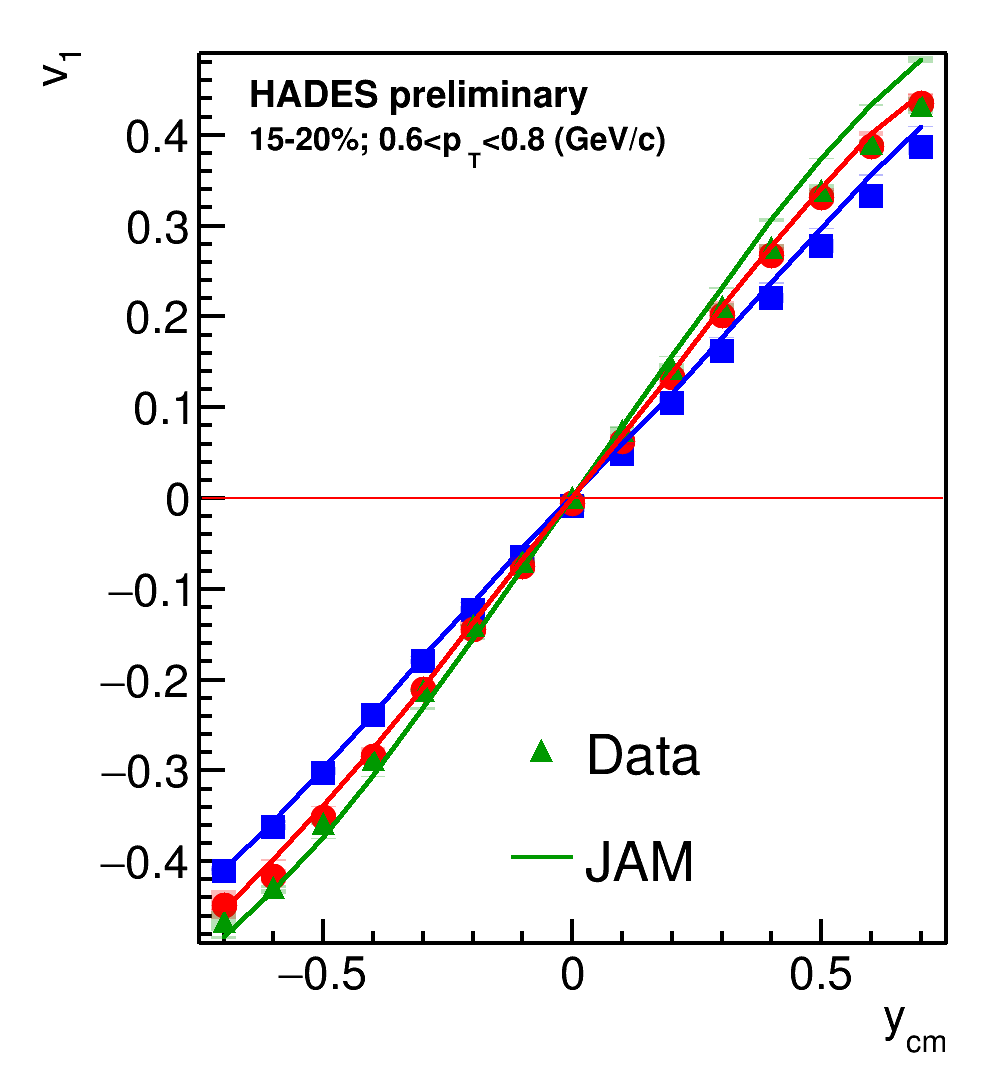
\includegraphics[width=0.45\linewidth]{images/v1_hades_ycm.png}
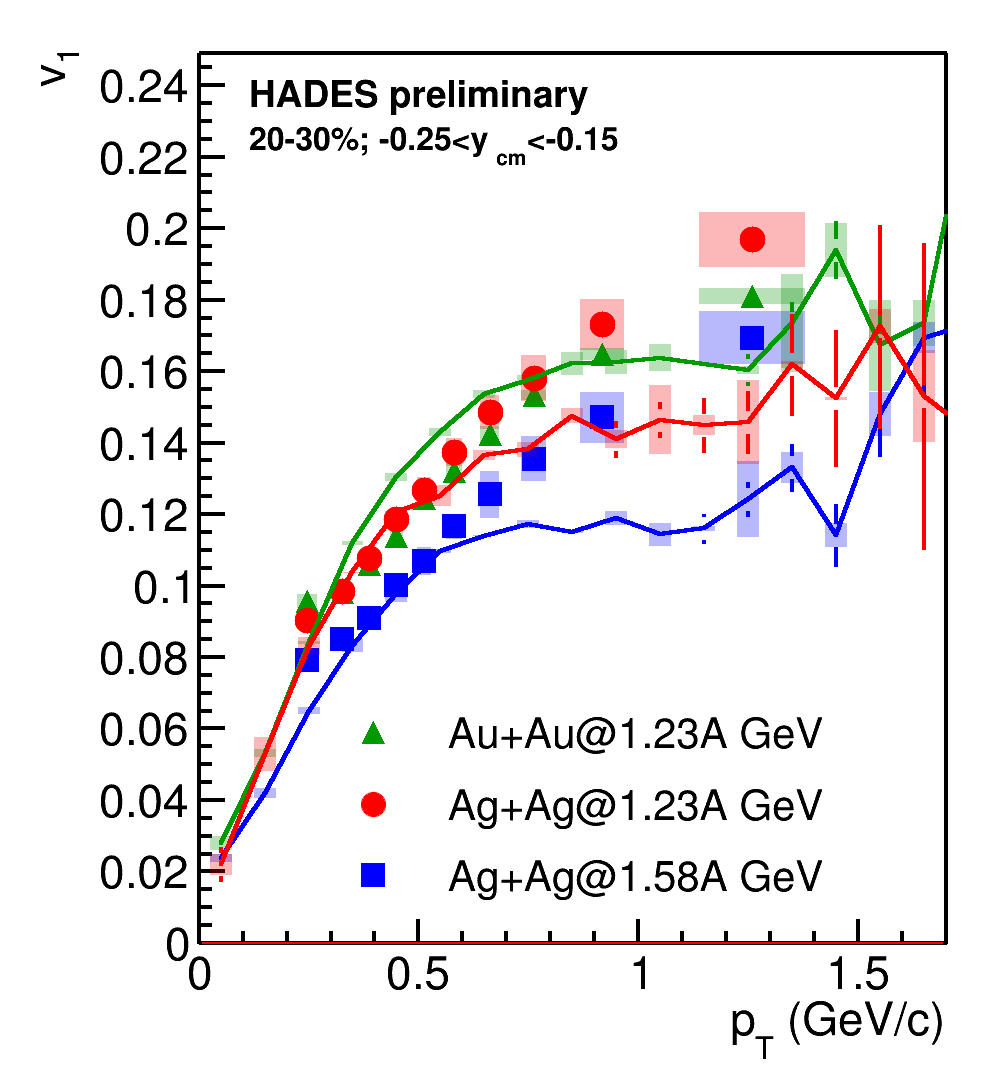
\includegraphics[width=0.45\linewidth]{images/v1_hades_pT.png}
\caption{Направленный поток протонов $v_1$ как фукция (справа) быстроты в системе центра масс $y_{cm}$ и (слева) поперечного импульса $p_T$ для столкновений Au+Au при энергии $E_{kin}=$1.23$A$~ГэВ и Ag+Ag при энергиях $E_{kin}=$1.23$A$ и 1.58$A$~ГэВ. Линиями показаны данные, полученные из модели JAM с импульсно-зависимым потенциалом.}
\label{fig:hades_v1_ycm_pT}
\end{center}
\end{figure}

\subsection{Проверка теоретических предсказаний эффектов масштабирования $v_1$ протнов в реалистичной модели Jet A-A Model (JAM)}

На рис.~\ref{fig:hades_model_ycm_scaling} представлены теоретические предсказания значений направленного потока протонов $v_1$ как функция быстроты столкновения $y_{cm}$ (слева) и быстроты, нормированной на быстроту пучка $y'=y_{cm}/y_{beam}$ (справа) из модели JAM.
Результаты для различных систем при одной энергии столкновения хорошо согласуются между собой и с экспериментальными данными для $v_1$ в столкновениях Au + Au при энергии $E_{kin}$=1.23$A$~ГэВ.
После нормировки быстроты столкновения на быстроту пучка, результаты можно описать единой кривой.
Этот факт свидетельствует о едином механизме образования направленного потока в данной области энергии в тяжелых системах.
%
\begin{figure}[ht]
\begin{center}
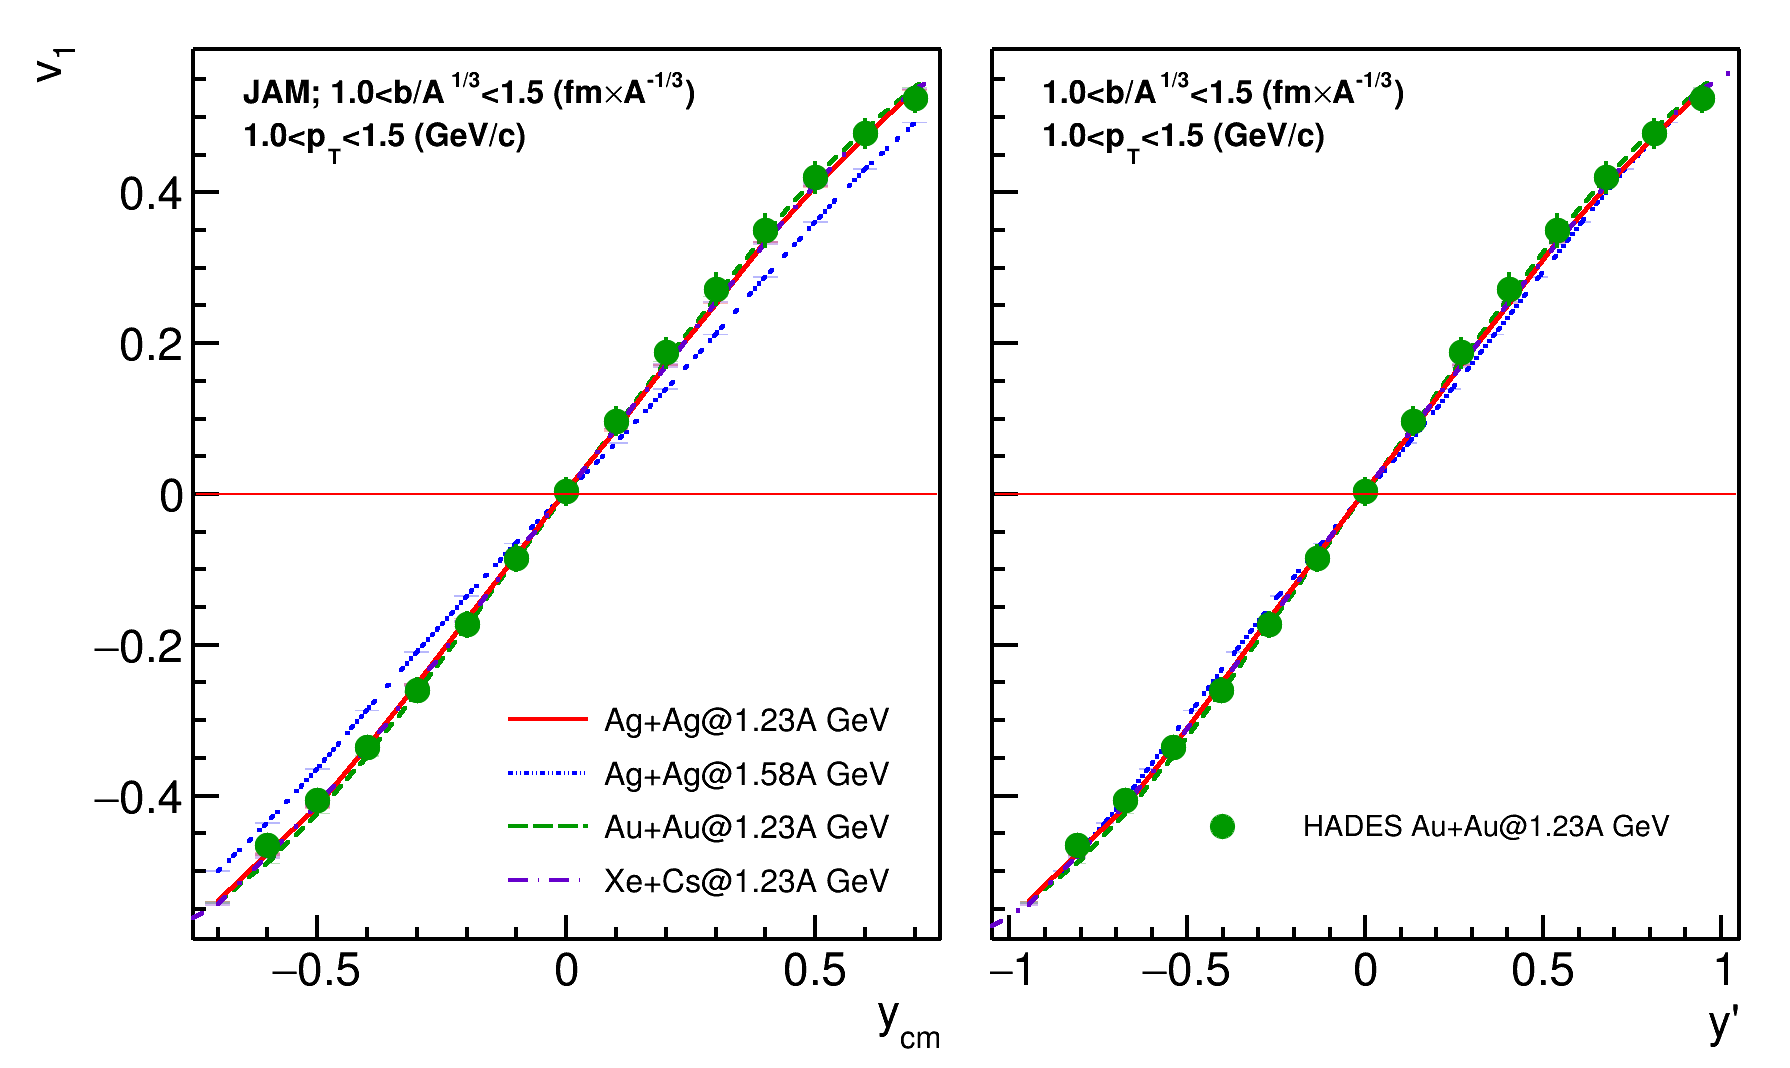
\includegraphics[width=0.95\linewidth]{images/v1_hades_model_ycm_scaling.png}
\caption{Направленный поток протонов $v_1$ как функция быстроты столкновения $y_{cm}$ (слева) и быстроты, нормированной на быстроту пучка $y'=y_{cm}/y_{beam}$ (справа) из модели JAM.}
\label{fig:hades_model_ycm_scaling}
\end{center}
\end{figure}

\subsection{Проверка эффектов масштабирования наклона направленного потока протонов в средних быстротах $dv_1/dy|_{y=0}$}

Зависимость направленного потока протонов $v_1$ как функция быстроты была параметризована кубической функцией $v_1(y_{cm}) = a_0 + a_1 y_{cm} + a_3 y_{cm}^3$. 
Затем наклон направленного потока протонов в нуле быстроты $dv_1/dy_{cm}|_{y_{cm}=0}$ был извлечен как параметр $a_1$.
На рис.~\ref{fig:hades_dv1dy_many_plot} слева приведена зависимость наклона направленного потока в нуле быстроты как функция центральности столкновения.
Наклоны $dv_1/dy_{cm}|_{y_{cm}=0}$ протонов для столкновений Au+Au и Ag+Ag при одной энергии хорошо согласуются между собой за исключением наиболее центральных событий. 
Поскольку c ростом энергии столкновения, время пролета уменьшается, наклон направленного потока протонов в столкновениях Ag+Ag при энергии $E_{kin}=$1.58$A$~ГэВ заметно меньше.
Для коррекции на время пролета, наклон направленного потока протонов $dv_1/dy_{cm}|_{y_{cm}=0}$ был нормирован на быстроту пучка $dv_1/dy_{cm}|_{y_{cm}=0} \times y_{b} = dv_1/dy'|_{y'=0}$, где $y_{b}$ --- быстрота пучка (0.74 для $E_{kin}=$1.23$A$~ГэВ и 0.82 для  $E_{kin}=$1.58$A$~ГэВ) и $y'=y_{cm}/y_b$.
Наклон направленного потока протонов нормированный на быстроту $dv_1/dy'|_{y'=0}$ пучка как функция центральности показан на рис.~\ref{fig:hades_dv1dy_many_plot} в центре. 
За исключением наиболее центральных событий, зависимость наклона от центральности описывается одной кривой для всех трех наборов данных.
В каждом классе центральности был вычислен средний прицельный параметр $\langle b \rangle$. 
Радиус ядра пропорционален корню кубическому из массового числа $r_N \propto A^{1/3}$.
Для устранения зависимости от размера сталкиваемых ядер, средний прицельный параметр в классе центральности был нормирован на $A^{1/3}$.
Наклон направленного потока протонов, нормированный на быстроту пучка $dv_1/dy'|_{y'=0}$ как функция относительного прицельного параметра  $ \langle b \rangle / A^{1/3}$ представлен на рис~\ref{fig:hades_dv1dy_many_plot} справа.
Данное преобразование улучшило согласие зависимостей наклона в центральных событиях. 
%
\begin{figure}[ht]
\begin{center}
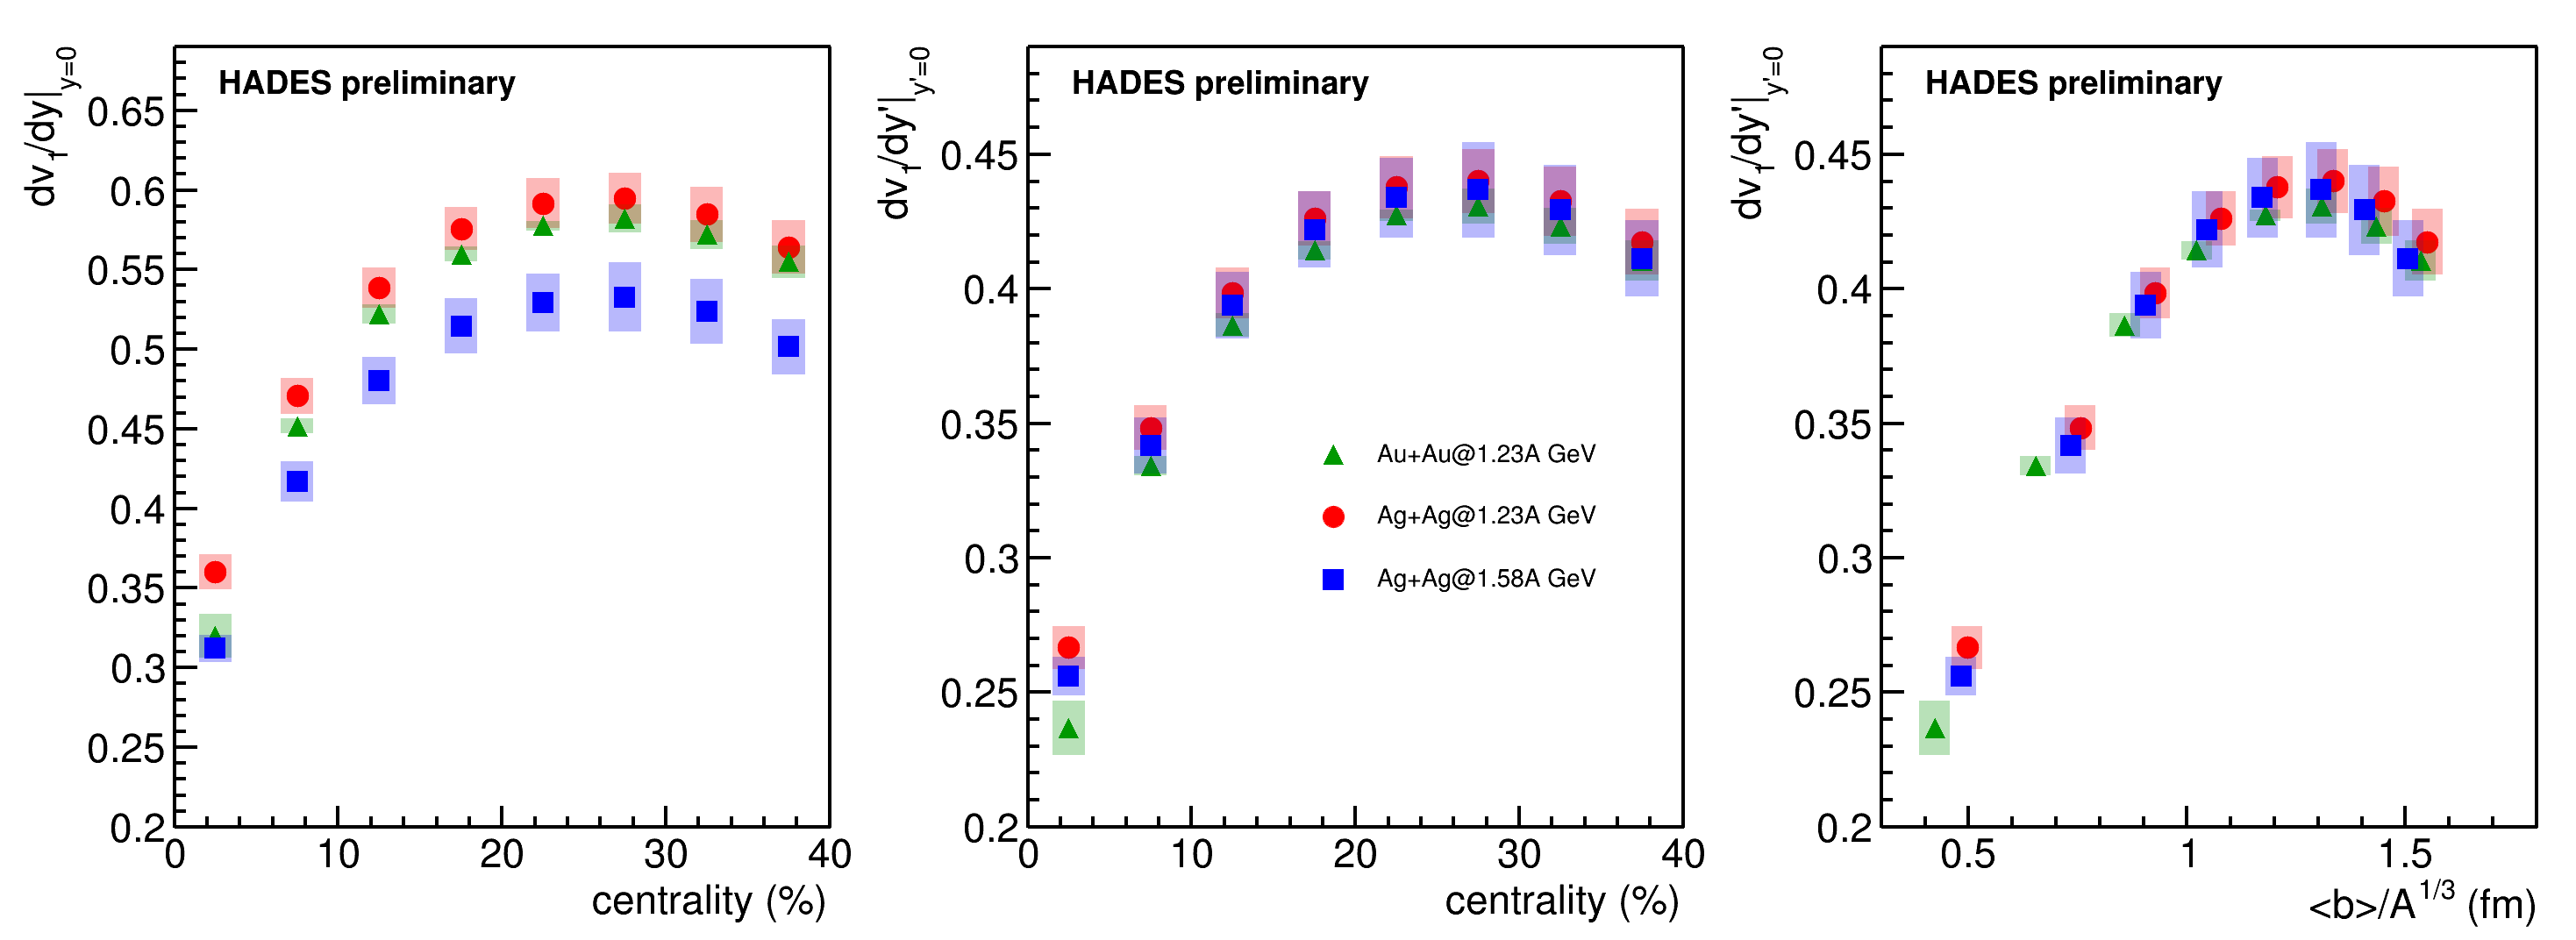
\includegraphics[width=0.9\linewidth]{images/dv1dy_many_plot.png}
\caption{ 
(Слева) Наклон направленного потока в нуле быстроты $dv_1/dy|_{y_{cm}=0}$ как функция центральности столкновений;
(посередине) наклон направленного потока в нуле быстроты нормированный на быстроту пучка $dv_1/dy|_{y'=0}$ как функция центральности столкновений;
(справа) наклон направленного потока в нуле быстроты нормированный на быстроту пучка $dv_1/dy|_{y'=0}$ как функция среднего прицельного параметра в классах центральности
для столкновений Au+Au при энергии $E_{kin}=$1.23$A$~ГэВ и Ag+Ag при энергиях $E_{kin}=$1.23$A$ и 1.58$A$~ГэВ. }
\label{fig:hades_dv1dy_many_plot}
\end{center}
\end{figure}

\subsection{Эффекты масштабирования для направленного потока $v_1$ протонов как функция поперечного импульса}

На рис.~\ref{fig:v1_pT_scaling} представлена зависимость от поперечного импульса $p_T$ направленного потока $v_1$ (слева) и направленного потока, нормированного на наклон в средних быстротах $v_1/dv_1/dy|_{y=0}$ (справа).
Результаты до нормировки для столкновений Au + Au и Ag + Ag при одной энергии находятся в хорошем согласии с учетом систематической ошибки.
Результаты для столкновений Ag + Ag при большей энергии систематически ниже, поскольку величина направленного потока $v_1$ зависит от времени пролета сталкивающихся ядер $t_{pass}$, которая меньше при более высокой энергии.
После нормировки (см. справа), все результаты ложатся на единую кривую.
Этот факт может свидетельствовать о едином механизме образования направленного потока в этой области энергии.
\begin{figure}[ht]
\begin{center}
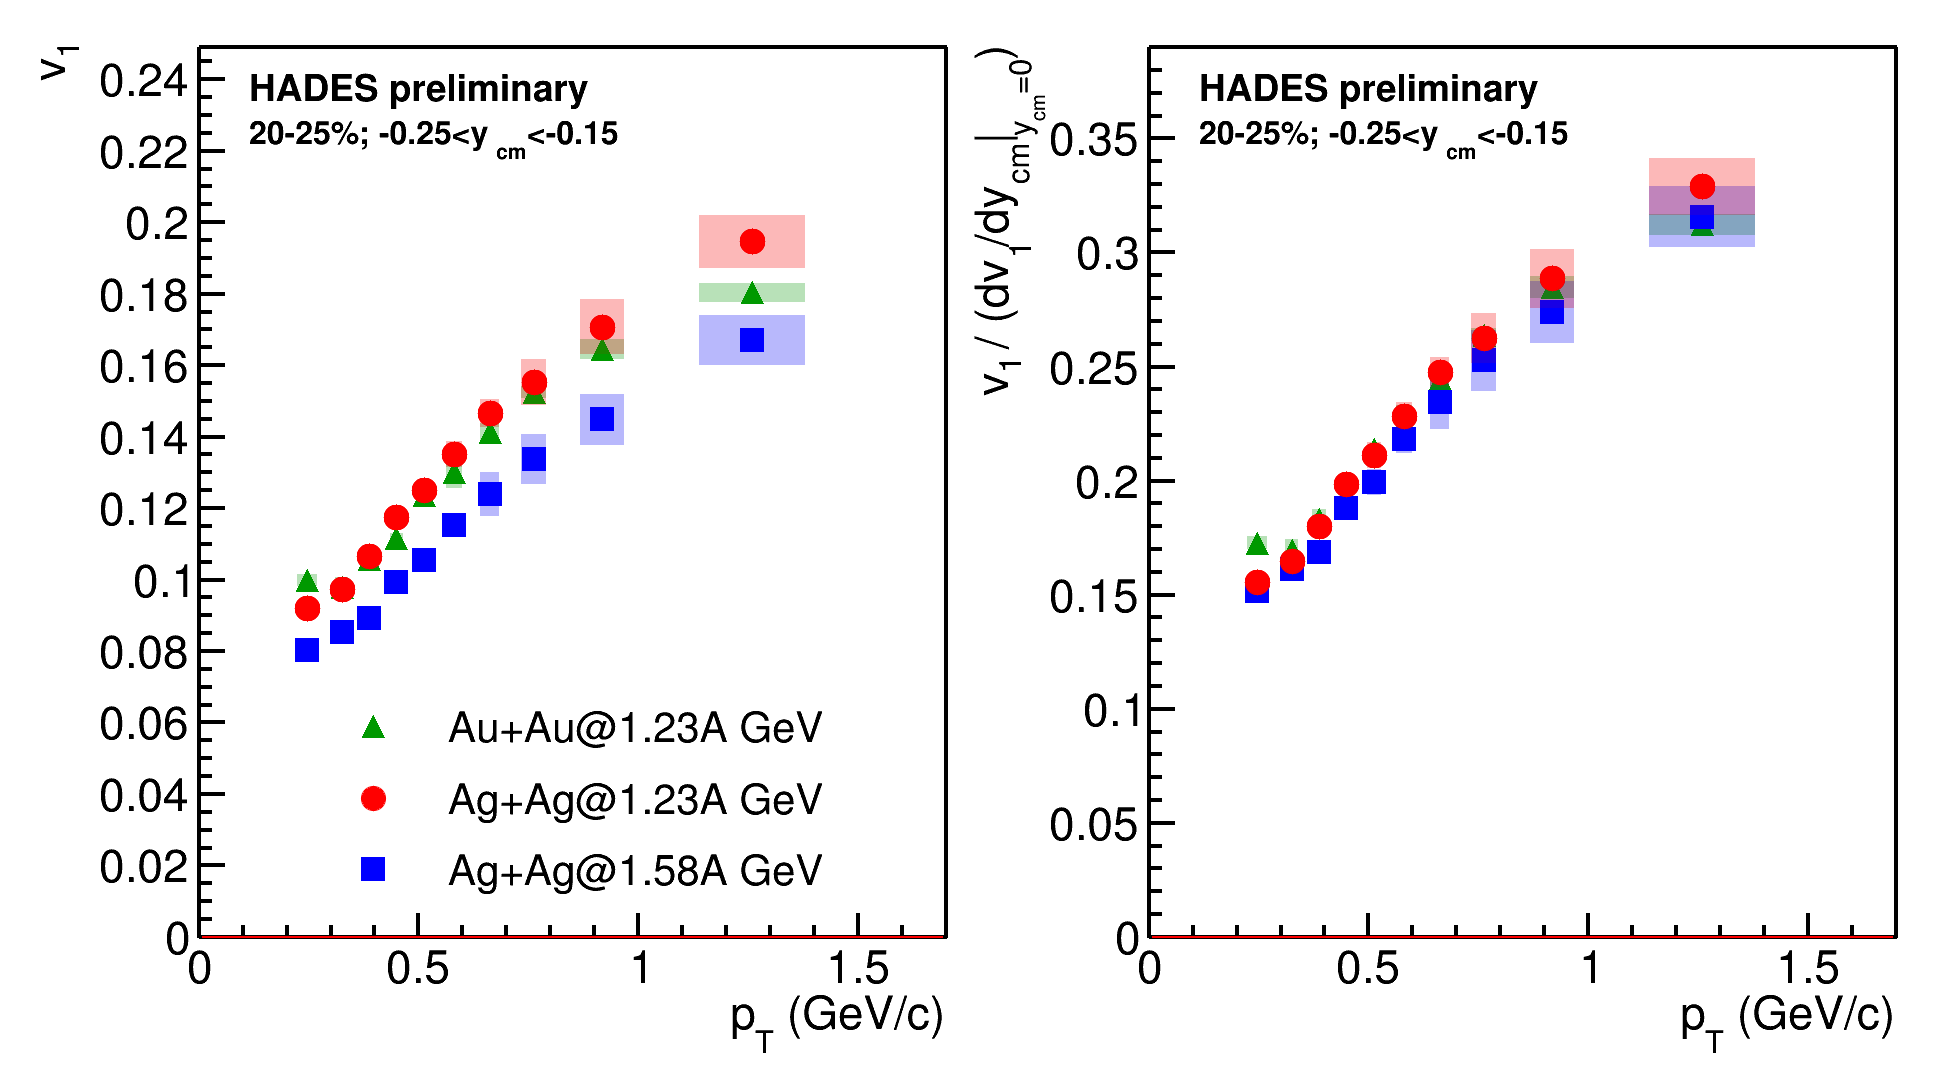
\includegraphics[width=0.9\linewidth]{images/v1_hades_pT_scaling.png}
\caption{ 
    Направленный поток протонов $v_1$ как функция поперечного импульса $p_T$. Слева: направленный поток $v_1$, справа: направленный поток, нормированный на наклон в средних быстротах $v_1/dv_1/dy|_{y=0}$.
}.
\label{fig:v1_pT_scaling}
\end{center}
\end{figure}

Описанный выше эффект был также обнаружен в модели с импульсно-зависимым потенциалом JAM.
На рис.~\ref{fig:v1_model_pT_scaling} представлена зависимость от поперечного импульса $p_T$ направленного потока $v_1$ (слева) и направленного потока, нормированного на наклон в средних быстротах $v_1/dv_1/dy|_{y=0}$ (справа) для различных систем из модели JAM.
До нормировки, результаты для направленного потока как функция $p_T$, для столкновений при одной энергии, находятся в довольно хорошем согласии.
После нормировки, теоретические предсказания для разных энергий и систем ложатся на единую кривую. 
\begin{figure}[ht]
\begin{center}
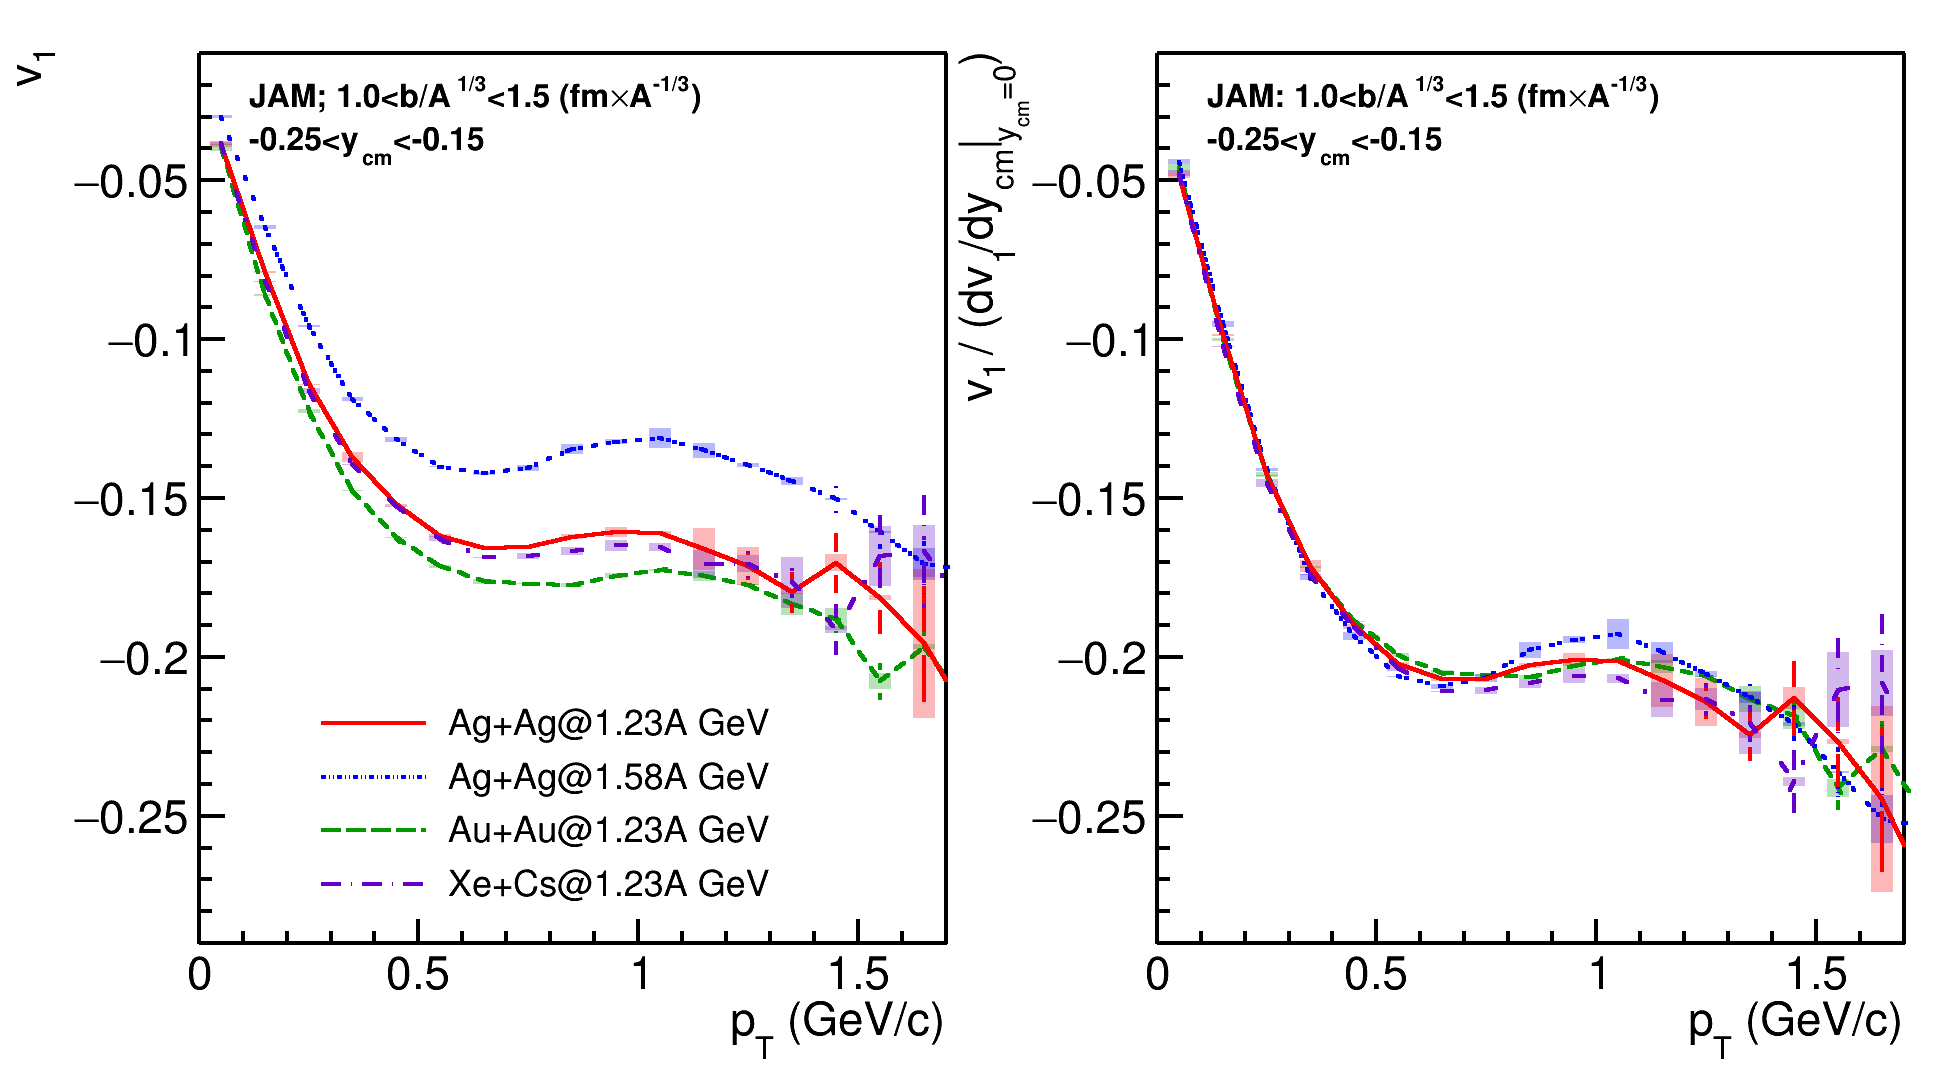
\includegraphics[width=0.9\linewidth]{images/v1_hades_model_pT_scaling.png}
\caption{ 
    Направленный поток протонов $v_1$ как функция поперечного импульса $p_T$ в модели JAM для различных сталкиваемых систем. Слева: направленный поток $v_1$, справа: направленный поток, нормированный на наклон в средних быстротах $v_1/dv_1/dy|_{y=0}$.
}.
\label{fig:v1_model_pT_scaling}
\end{center}
\end{figure}

\subsection{Сравнение измеренного наклона направленного потока протонов в средних быстротах с мировыми данными}

Сравнение полученных значений наклона направленного потока протонов $dv_1/dy|_{y_{cm}=0}$ с существующими результатами показано на рис.~\ref{fig:hades_dv1_dy_sqrt_snn}.
Значения $dv_1/dy|_{y_{cm}=0}$ протонов в столкновениях \au{} при $E_{kin}=$1.23$A$~ГэВ и \ag{} при $E_{kin}=$1.23$A$ и  при $E_{kin}=$1.58$A$~ГэВ согласуются с измерениями с ранее доступными данными с других экспериментов.
%
\begin{figure}[ht]
\begin{center}
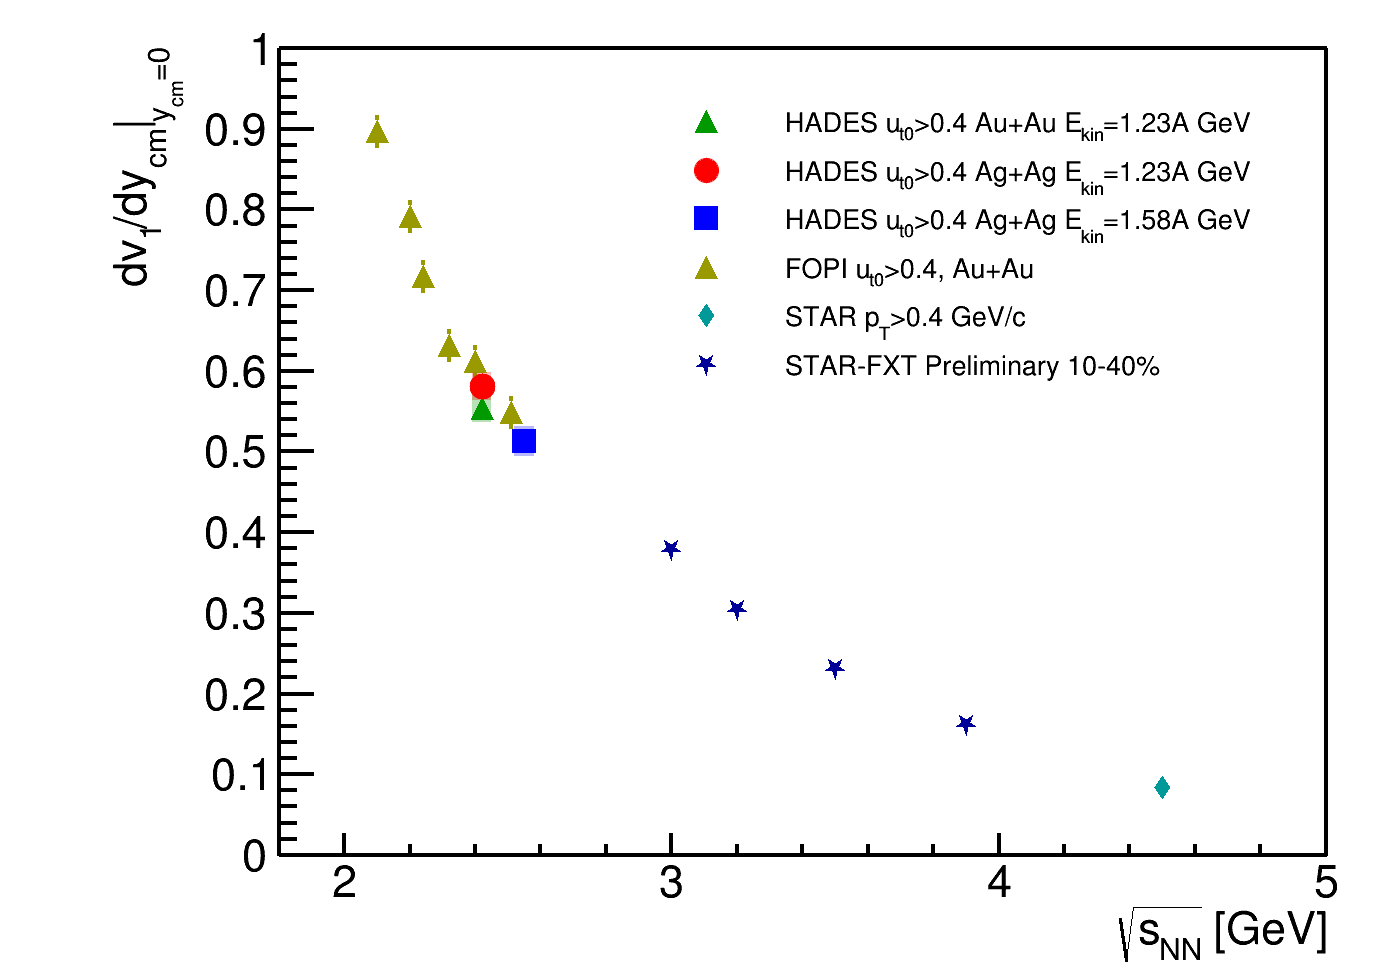
\includegraphics[width=0.9\linewidth]{images/dv1_dy_sqrt_snn.png}
\caption{ 
    Направленный поток протонов $dv_1/dy|_{y_{cm}=0}$ как функция энергии столкновения $\sqrt{s_{NN}}$. Экспериментальные значения наклона направленного потоа были взяты из следующих публикаций: E895~\cite{E895:2000maf}, FOPI~\cite{FOPI:2011aa}, STAR~\cite{STAR:2020dav}.
}
\label{fig:hades_dv1_dy_sqrt_snn}
\end{center}
\end{figure}